\appendix

\chapter{INSTALLATION GUIDE}
\label{app:installation}

This appendix provides comprehensive step-by-step instructions for setting up the CRM System development environment from scratch on any developer workstation (Windows, macOS, or Linux).

\section{Prerequisites}
Ensure the following software packages are installed on your workstation:
\begin{itemize}
    \item \textbf{Node.js:} Version 20.x LTS or higher (\url{https://nodejs.org/})
    \item \textbf{npm:} Version 9.x or higher (packaged automatically with Node.js)
    \item \textbf{Git:} Version 2.40 or higher (\url{https://git-scm.com/})
    \item \textbf{Docker Desktop:} (Optional, for containerized local execution)
\end{itemize}

\section{Repository Cloning}
Clone the project repository from GitHub and navigate to the project directory:
\begin{lstlisting}[language=bash]
# Clone repository via HTTPS
git clone https://github.com/Kowshik1759/CRM-System.git

# Enter project root directory
cd CRM-System
\end{lstlisting}

\section{Backend Dependencies and Environment Configuration}
Navigate into the \texttt{backend/} directory and install dependencies:
\begin{lstlisting}[language=bash]
cd backend
npm install
\end{lstlisting}

Create a local environment file named \texttt{.env} inside the \texttt{backend/} folder based on \texttt{.env.example}:
\begin{lstlisting}[language=bash]
# backend/.env configuration
PORT=5000
NODE_ENV=development
MONGO_URI=mongodb+srv://<username>:<password>@cluster0.xxxxx.mongodb.net/crm_db?retryWrites=true&w=majority
JWT_SECRET=crm_super_secret_jwt_key_2026_production
JWT_EXPIRES_IN=7d
\end{lstlisting}
*(Note: If no \texttt{MONGO\_URI} is supplied in development mode, the backend automatically initializes an in-memory embedded MongoDB database for local testing).*

\section{Frontend Dependencies Configuration}
Navigate into the \texttt{frontend/} directory and install the client dependencies:
\begin{lstlisting}[language=bash]
cd ../frontend
npm install
\end{lstlisting}

% ==============================================================================
\chapter{APPLICATION EXECUTION GUIDE}
\label{app:execution}

\section{Running in Local Development Mode}
The CRM System provides automated runners to launch both backend and frontend services concurrently:

\subsection{Concurrent Runner (Cross-Platform)}
From the root directory of the project, execute:
\begin{lstlisting}[language=bash]
npm run dev
\end{lstlisting}
This command triggers \texttt{start-dev.js}, which concurrently spawns:
\begin{itemize}
    \item Express API server on \url{http://localhost:5000}
    \item Vite React development client on \url{http://localhost:3000}
\end{itemize}

\subsection{Windows PowerShell Launcher}
On Windows workstations, execute the provided PowerShell script:
\begin{lstlisting}[language=bash]
.\start-dev.ps1
\end{lstlisting}

\section{Accessing the System and Demo Credentials}
Once launched, navigate your browser to \url{http://localhost:3000} (or the production URL). The system provides four built-in demo personas for immediate testing:

\begin{table}[h!]
\centering
\caption{Pre-Configured System Demo Credentials}
\label{tab:demo_creds}
\renewcommand{\arraystretch}{1.3}
\begin{tabular}{|p{3.5cm}|p{5cm}|p{3cm}|p{3cm}|}
\hline
\textbf{Role} & \textbf{Email Address} & \textbf{Password} & \textbf{Default Landing} \\ \hline
\textbf{Admin} & \texttt{admin@crm.com} & \texttt{Admin@123} & Executive Dashboard \\ \hline
\textbf{Sales Manager} & \texttt{manager@crm.com} & \texttt{Manager@123} & Executive Dashboard \\ \hline
\textbf{Sales Executive} & \texttt{sales@crm.com} & \texttt{Sales@123} & Sales Pipeline \\ \hline
\textbf{Customer Support} & \texttt{support@crm.com} & \texttt{Support@123} & Customers Registry \\ \hline
\end{tabular}
\end{table}

\section{Running with Docker Compose}
To execute the complete application inside isolated Docker containers (including a persistent MongoDB database container):
\begin{lstlisting}[language=bash]
# Build and launch all three containers in detached mode
docker-compose up --build -d

# Verify container health status
docker-compose ps

# Access frontend at http://localhost:3000
# Access backend at http://localhost:5000/api/health
\end{lstlisting}

% ==============================================================================
\chapter{API REFERENCE}
\label{app:api}

The table below outlines the core REST API contract exposed by the backend service. All endpoints except \texttt{/health} and \texttt{/api/v1/auth/login} require a valid Bearer token in the \texttt{Authorization} HTTP header.

\begin{table}[h!]
\centering
\caption{Summary of REST API Resources}
\renewcommand{\arraystretch}{1.2}
\begin{tabular}{|p{1.5cm}|p{4.5cm}|p{3cm}|p{5cm}|}
\hline
\textbf{Verb} & \textbf{Path} & \textbf{Auth Required?} & \textbf{Functionality} \\ \hline
\texttt{GET} & \texttt{/health} & No & Public server health status probe \\ \hline
\texttt{POST} & \texttt{/api/v1/auth/login} & No & Authenticates credentials; returns JWT \\ \hline
\texttt{GET} & \texttt{/api/v1/auth/me} & Yes (All) & Retrieves active user session \\ \hline
\texttt{GET} & \texttt{/api/v1/dashboard} & Yes (All) & Aggregates real-time business KPIs \\ \hline
\texttt{GET} & \texttt{/api/v1/customers} & Yes (All) & Retrieves searchable customer accounts \\ \hline
\texttt{POST} & \texttt{/api/v1/customers} & Yes (Admin, Mgr, Exec) & Creates new customer record \\ \hline
\texttt{GET} & \texttt{/api/v1/leads} & Yes (Admin, Mgr, Exec) & Retrieves lead registry with filters \\ \hline
\texttt{POST} & \texttt{/api/v1/leads/:id/convert} & Yes (Admin, Mgr, Exec) & Converts lead to customer record \\ \hline
\texttt{GET} & \texttt{/api/v1/pipeline} & Yes (Admin, Mgr, Exec) & Returns deals grouped by Kanban stages \\ \hline
\texttt{GET} & \texttt{/api/v1/tasks} & Yes (All) & Retrieves delegated operational tasks \\ \hline
\texttt{GET} & \texttt{/api/v1/followups} & Yes (All) & Lists upcoming and overdue follow-ups \\ \hline
\texttt{GET} & \texttt{/api/v1/interactions} & Yes (All) & Chronological client communication logs \\ \hline
\texttt{GET} & \texttt{/api/v1/reports/*} & Yes (Admin, Mgr) & Generates 4 analytical reports \\ \hline
\texttt{GET} & \texttt{/api/v1/users} & Yes (Admin Only) & Employee user administration \\ \hline
\end{tabular}
\end{table}

% ==============================================================================
\chapter{DATABASE SCHEMA}
\label{app:schema}

The MongoDB document schema definitions are enforced via Mongoose models located under \texttt{backend/src/models/}:
\begin{itemize}
    \item \textbf{\texttt{User.js}:} Stores employee accounts, hashed passwords, roles, and status flags.
    \item \textbf{\texttt{Customer.js}:} Stores customer profiles, corporate accounts, contact details, and assigned representatives.
    \item \textbf{\texttt{Lead.js}:} Captures inbound sales leads, lead channels, qualification stages, and deal scores.
    \item \textbf{\texttt{Opportunity.js}:} Tracks deal values, closing probabilities, and stage-gate milestones.
    \item \textbf{\texttt{Task.js}:} Manages operational tasks, priority flags, deadlines, and employee delegations.
    \item \textbf{\texttt{FollowUp.js}:} Coordinates meetings, calls, and email follow-ups with reminder intervals.
    \item \textbf{\texttt{Interaction.js}:} Documents client communication entries, notes, and outcomes.
\end{itemize}

% ==============================================================================
\chapter{GITHUB REPOSITORY INFORMATION}
\label{app:github}

\begin{itemize}
    \item \textbf{Repository URL:} \url{https://github.com/Kowshik1759/CRM-System}
    \item \textbf{Default Branch:} \texttt{master}
    \item \textbf{Owner:} Kowshik1759
    \item \textbf{License:} MIT Open Source License
    \item \textbf{Repository Topics:} crm, mern-stack, react, vite, nodejs, express, mongodb-atlas, tailwindcss, devops, docker, kubernetes, vercel, render
    \item \textbf{Repository Structure:} Decoupled frontend (\texttt{frontend/}), backend REST service (\texttt{backend/}), and cloud orchestration manifests (\texttt{k8s/}).
\end{itemize}

% ==============================================================================
\chapter{DEPLOYMENT INFORMATION}
\label{app:deployment}

The production deployment of the CRM System is distributed across three specialized cloud providers:

\begin{table}[h!]
\centering
\caption{Production Cloud Deployment Architecture Details}
\renewcommand{\arraystretch}{1.3}
\begin{tabular}{|p{3cm}|p{3.5cm}|p{7.5cm}|}
\hline
\textbf{Subsystem} & \textbf{Cloud Platform} & \textbf{Production Endpoint / Configuration} \\ \hline
\textbf{Frontend SPA} & Vercel Edge Hosting & \url{https://crm-system-sable-delta.vercel.app} \newline
Vite build, global edge CDN, automatic HTTPS \\ \hline
\textbf{Backend API} & Render Cloud Web Service & \url{https://crm-system-ea6d.onrender.com} \newline
Node.js runtime, automated restarts, dynamic port binding \\ \hline
\textbf{Database} & MongoDB Atlas & Cloud cluster \texttt{crm\_db} \newline
Replica set persistence, automated snapshots, TLS encrypted \\ \hline
\textbf{Health Probe} & Render / Public Endpoint & \url{https://crm-system-ea6d.onrender.com/health} \newline
Returns HTTP 200 with service uptime statistics \\ \hline
\end{tabular}
\end{table}

% ==============================================================================
\chapter{SCREENSHOTS OF IMPLEMENTED MODULES}
\label{app:screenshots}

This appendix documents the primary visual user interfaces and cloud dashboards of the deployed CRM application.

\begin{figure}[h!]
\centering
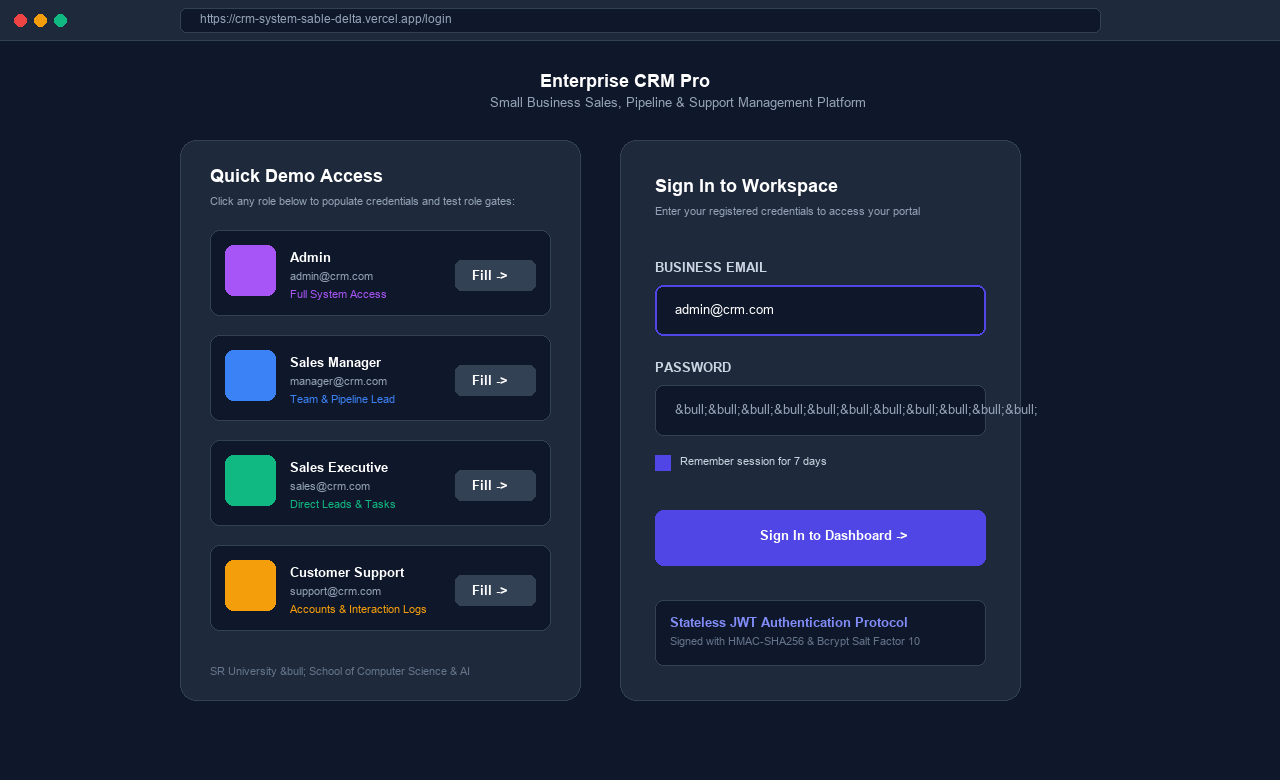
\includegraphics[width=0.95\textwidth]{figures/screen_login.png}
\caption{Authentication Interface: Multi-Role Sign-In and Demo Quick-Fill Access Cards}
\label{fig:app_login}
\end{figure}

\begin{figure}[h!]
\centering
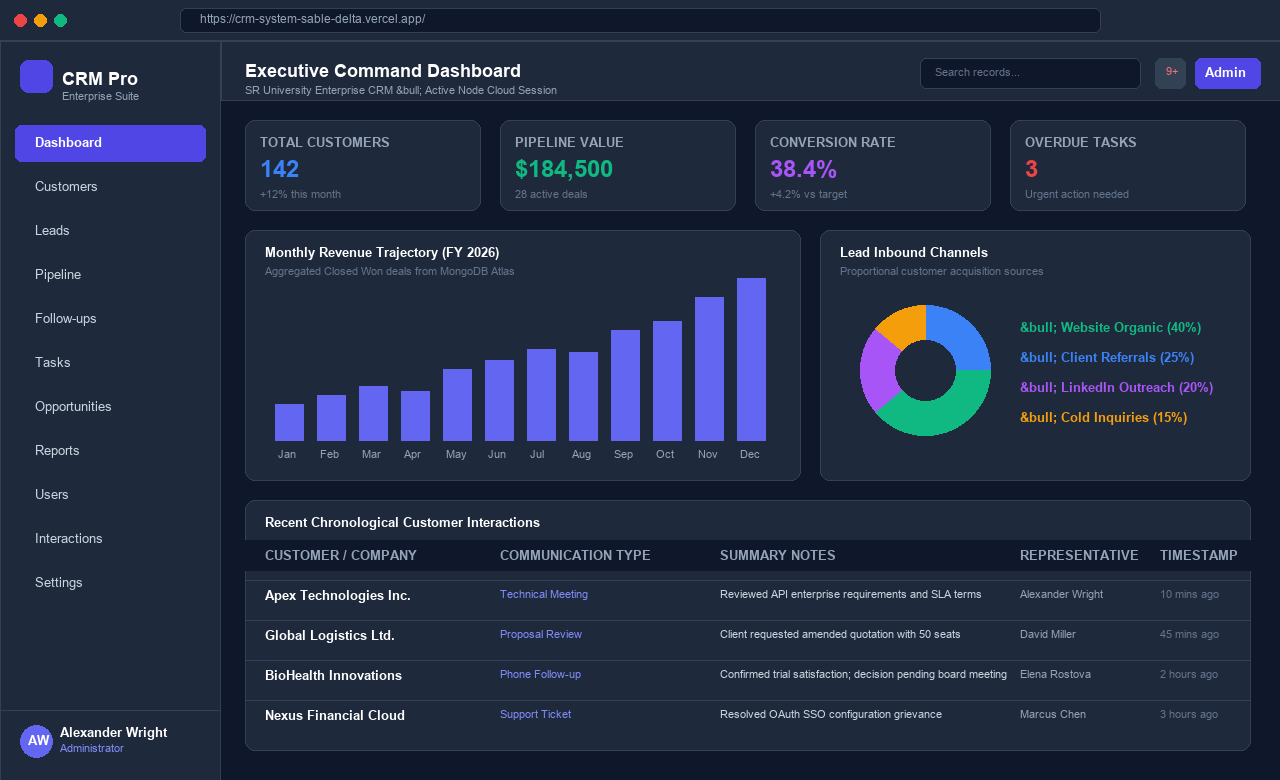
\includegraphics[width=0.95\textwidth]{figures/screen_dashboard.png}
\caption{Executive Command Dashboard: Real-Time Business KPIs and Recharts Trajectory Analytics}
\label{fig:app_dashboard}
\end{figure}

\begin{figure}[h!]
\centering
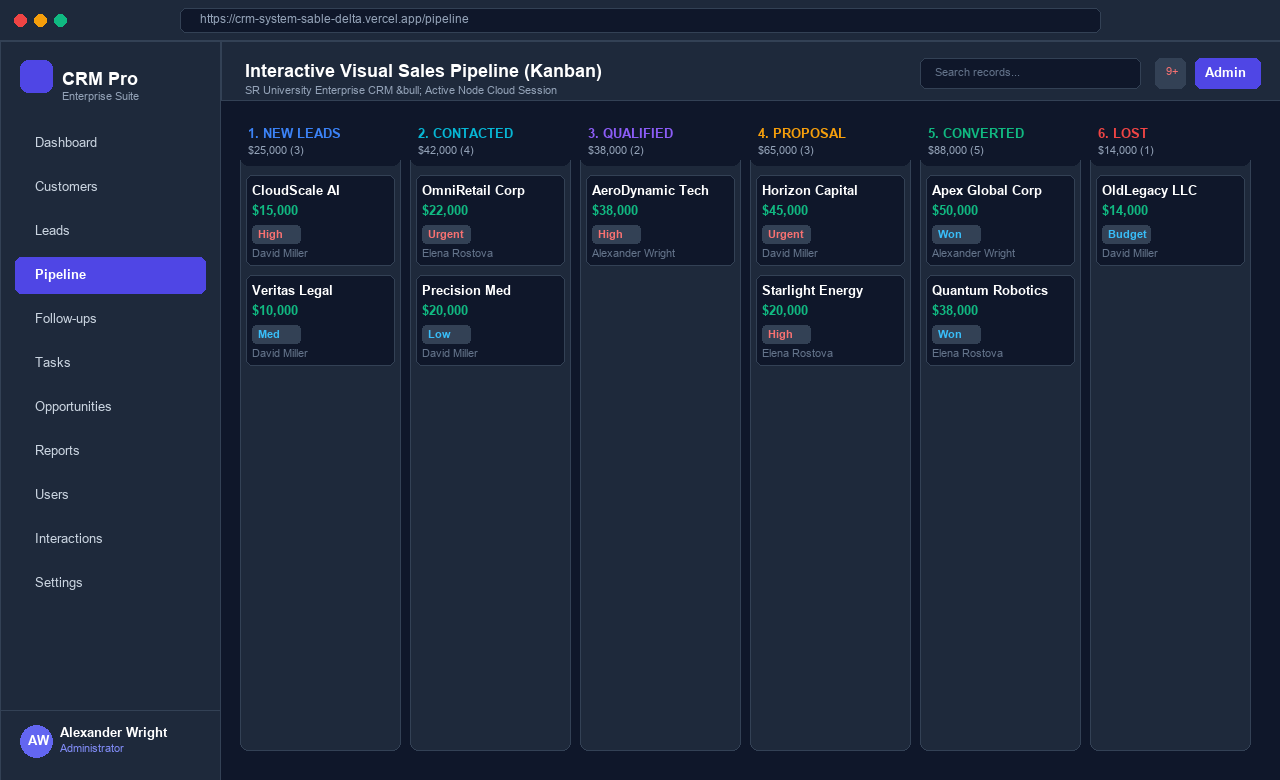
\includegraphics[width=0.95\textwidth]{figures/screen_pipeline.png}
\caption{Interactive Kanban Sales Pipeline: Visual Stage-Gate Commercial Deal Board}
\label{fig:app_pipeline}
\end{figure}

\begin{figure}[h!]
\centering
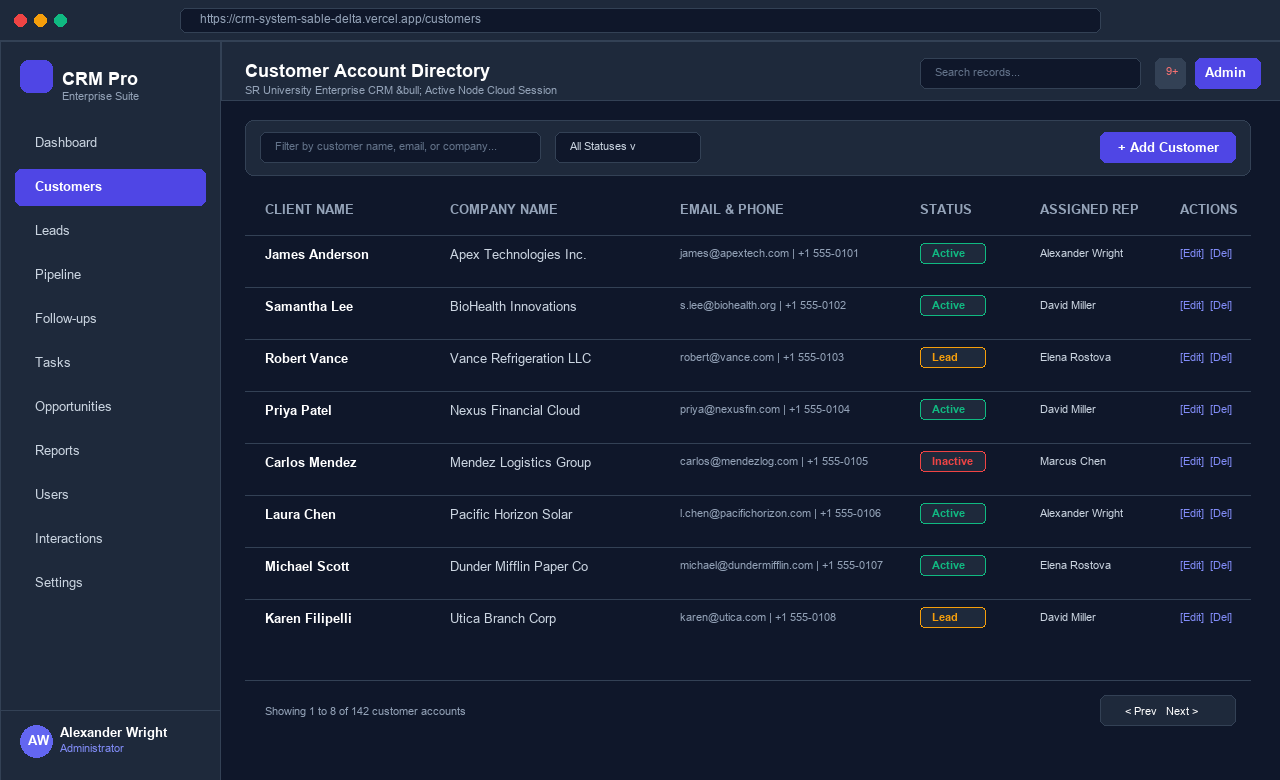
\includegraphics[width=0.95\textwidth]{figures/screen_customers.png}
\caption{Customer Account Directory: Multi-Criteria Filter, Status Badges, and Account Table}
\label{fig:app_customers}
\end{figure}

\begin{figure}[h!]
\centering
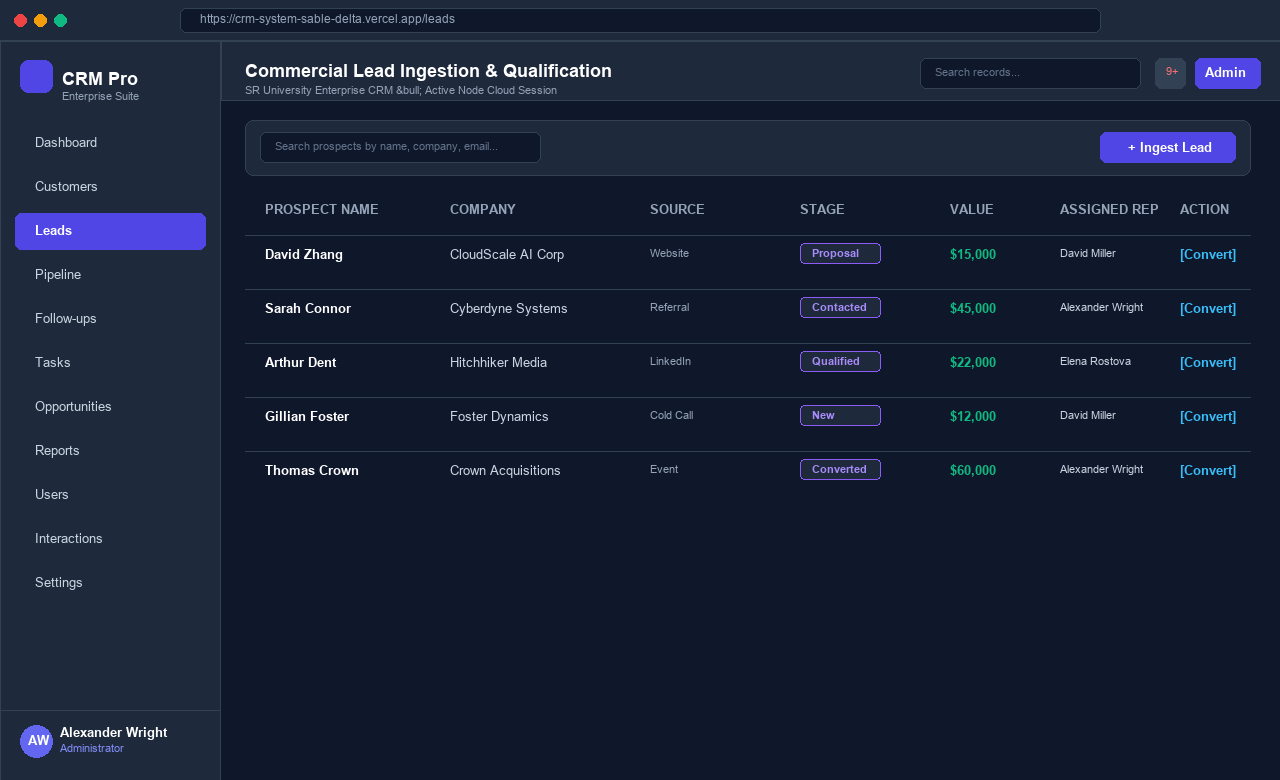
\includegraphics[width=0.95\textwidth]{figures/screen_leads.png}
\caption{Commercial Lead Ingestion and Qualification Console}
\label{fig:app_leads}
\end{figure}

\begin{figure}[h!]
\centering
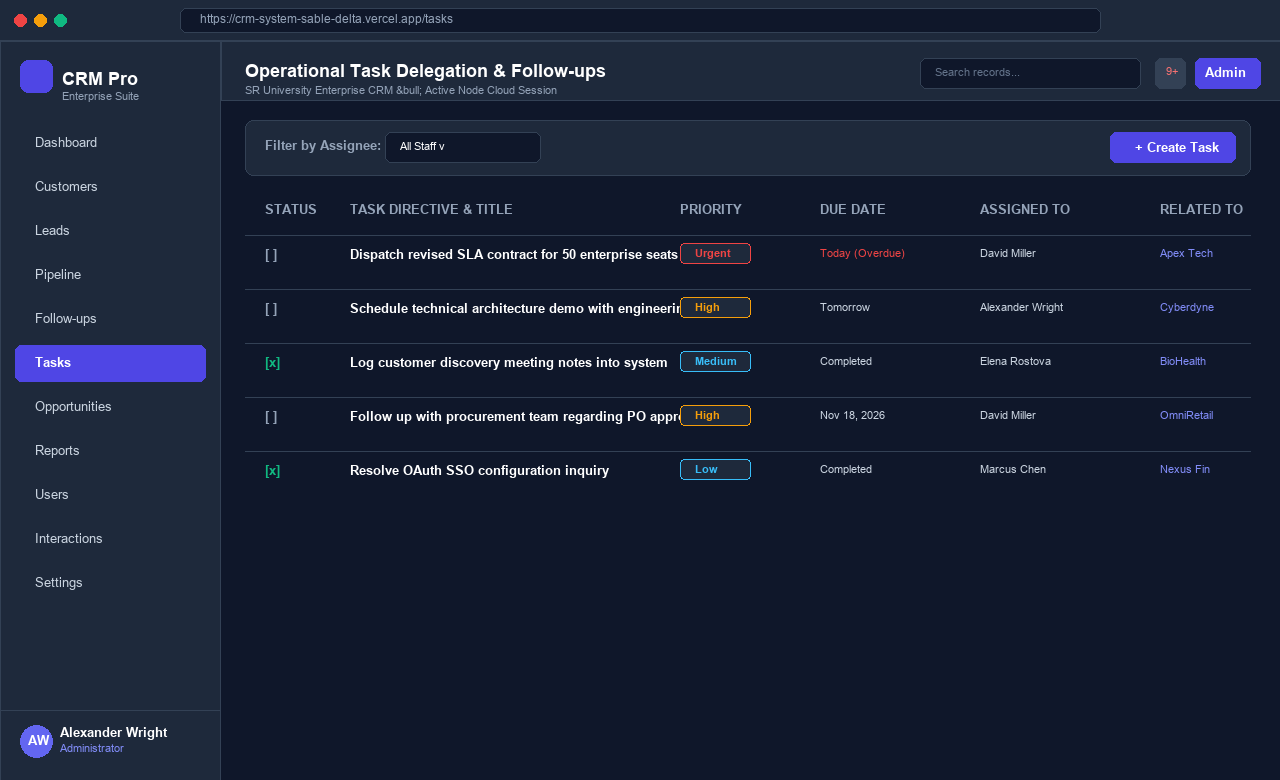
\includegraphics[width=0.95\textwidth]{figures/screen_tasks.png}
\caption{Operational Task Management Board with Deadline Status and Priority Indicators}
\label{fig:app_tasks}
\end{figure}

\begin{figure}[h!]
\centering
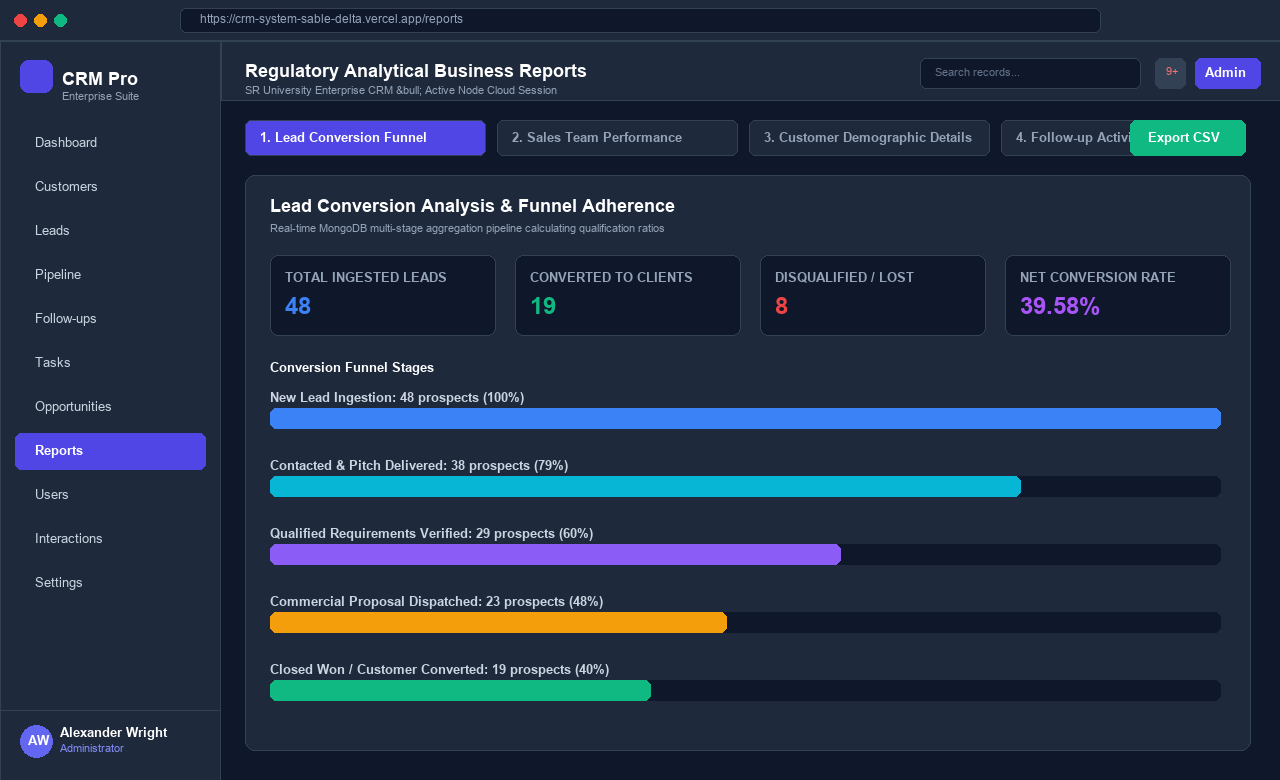
\includegraphics[width=0.95\textwidth]{figures/screen_reports.png}
\caption{Regulatory Analytical Reports Suite: Dynamic Funnel Breakdown and CSV Export}
\label{fig:app_reports}
\end{figure}

\begin{figure}[h!]
\centering
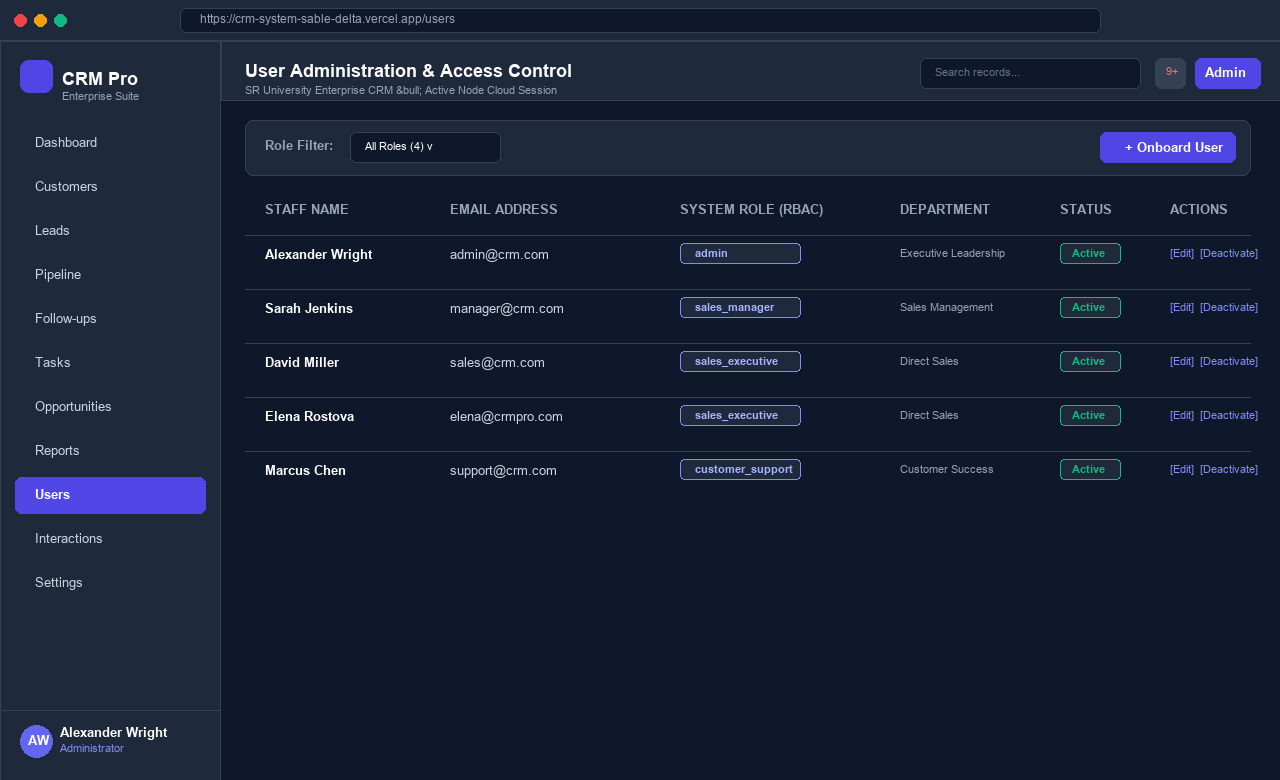
\includegraphics[width=0.95\textwidth]{figures/screen_users.png}
\caption{Administrator Staff Directory and Role-Based Access Control Console}
\label{fig:app_users}
\end{figure}
